\documentclass[12pt]{article}
\usepackage[francais]{babel}
\usepackage[utf8]{inputenc}
\usepackage{glossaries}
\makeglossaries
\usepackage{color}
\usepackage{graphicx}
\usepackage{amsmath}
\usepackage{amssymb}
\usepackage{mathrsfs}
\usepackage{listings}
\usepackage{textcomp}
\usepackage{fancyhdr}
\usepackage{eurosym}
\pagestyle{fancy}

\newglossaryentry{computer}
{
  name=computer,
  description={is a programmable machine that receives input,
               stores and manipulates data, and provides
               output in a useful format}
}

\newcommand{\HRule}{\rule{\linewidth}{0.5mm}}

\fancyhead[L]{}
\fancyhead[R]{}
\fancyfoot[R]{
\includegraphics [width=4cm]{logo.jpg}}
\renewcommand{\headrulewidth}{0pt}

\begin{document}

\renewcommand{\glossaryname}{Glossaire}

\begin{titlepage}
	\begin{center}

		\HRule \\[0.4cm]
		{ \huge \bfseries Rapport de projet - Dawn of Gates\\[0.4cm] }
		\HRule \\[2cm]


		\large \textsc 0\_Dev Team\\
		\textsc{Lariau} Steven (lariau\_s) \\
		\textsc{Brenet} Timothée (brenet\_t)\\
		\textsc{Lafargue} Victor (lafarg\_b)\\

		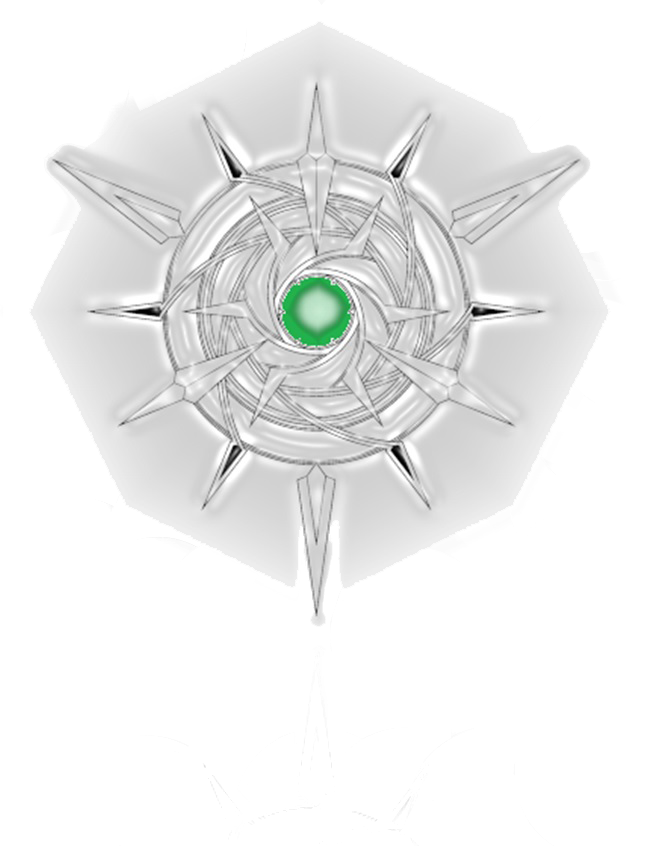
\includegraphics[scale=0.45]{logo2.png}
		
		\large \textsc Epita S2 - XX/06/15

	\end{center}
\end{titlepage}

\newpage

\section*{Remerciements}

De \gls{computer} nombreuses personnes nous ont apportés de l'aide dans la la réalisation de notre projet, sans la communité du forum d'unity pour le jeu et de stack overflow pour le c\# en général et le site nous n'aurions pu faire face à tous les problèmes rencontrés lors du développement.\\
Nous tenons aussi à remercier HTML5Up, le site web sur lequel nous avons été cherché le template css pour notre site web.

\newpage

\section*{Introduction}

A l'origine, il a été choisi unanimement que nous développerions un jeu-vidéo. Inspirés du fameux jeu Portal, il nous est venu l'idée de créer un concept de jeu innovant autour des portes de téléportation mais sur un concept fondamentalement différent à celui de Portal bien sûr. D'où le nom Dawn Of Gates.\\
L'un de nous disposant du casque de réalité virtuelle Oculus Rift, nous avons choisi de nous lancer dans la création d'un jeu en réalité virtuelle. Nous avons fait ce choix pour apporter une touche d'originalité au jeu mais aussi pour donner au joueur une réelle sensation d'immersion au sein de notre jeu. Notre choix est aussi dû au fait que le casque Oculus Rift est un bijou de technologie qui permet une immersion totale dans le jeu. Il présente l'avantage de profiter d'une vue à la première personne à 360degres. C'est-à-dire que nous percevons l'environnement qui nous entoure sous tous les angles avec une impression 3D saisissante. Nous aimons les perspectives d'un tel outil et c'est pourquoi nous tenions à travailler dessus.\\
Nous avons ensuite élaboré les premières bases de notre jeu. Le personnage principal, celui du joueur est un ninja. Il a la capacité de lancer des shurikens (petites armes que l'on lance) sur les murs. Ces shurikens une fois arrivés sur le mur se transforment en porte de téléportation. Les portes de téléportation remplissent un rôle majeur dans le jeu. Le joueur a aussi la possibilité de ralentir le temps dans certaines occasions en appuyant sur une touche. Ces deux éléments forment le concept principal du jeu sur lequel est basé le gameplay du jeu.\\

Le but de ce projet était de réaliser un projet qui nous tenais à cœur : la réalisation d'un véritable jeu-vidéo. C'est d'ailleurs cette motivation qui nous a permis de réussir notre projet. Outre la réalisation en elle-même, l'intérêt du projet est aussi de développer nos compétences techniques qui nous permettrons plus tard d'exercer notre futur métier. Enfin ce projet a aussi pour but de exercer notre capacité à travailler en équipe pour plus tard mener à bien de réels projets avec enjeux financiers et contraintes horaires dans le monde du travail.\\
Notre organisation était au début construite pour fonctionner avec quatre personnes mais suite au départ d'Idris, nous avons dû changer notre organisation. Les réalisations graphiques tels que les modélisations, les poses de textures et les animations et quelques scripts étaient faites par Victor. L'intelligence artificielle des ennemis et plusieurs autres scripts étaient fait par Timothée. Le capacité de slow motion et plusieurs autres scripts étaient réalisée par Steven.\\\\

Dans un premier temps, nous ferons la présentation générale de notre jeu en rappelant les principaux éléments constitutifs du gameplay. Nous présenterons ensuite les différents membres de l'équipe et l'organisation générale du projet. Puis nous détaillerons tout ce qui est relatif au personnage principal, celui que le joueur contrôle. Dans la quatrième partie, nous expliquerons le fonctionnement des niveaux. Nous présenterons ensuite les différents niveaux. Après cela, nous parlerons du mode multijoueur qui est la principale innovation de la troisième soutenance. Le site web sera ensuite présenté. Enfin nous ferons chacun nos conclusions personnelles.


\newpage

\renewcommand{\contentsname}{Sommaire}
\tableofcontents

\newpage

\section{Présentation du projet}

\subsection{Un jeu en réalité virtuelle}

Dawn of Gates est un jeu en réalité virtuelle, cela signifie que le joueur ne se contente pas seulement de jouer devant son écran, il est réellement émergé dans le jeu. Il met un casque sur sa tête, possédant deux écran, un pour chaque oeil, ayant pour but de faire croire au joueur que celui-ci est réellement dans le jeu.\\
Il existe plusieurs modèles de casques de réalité virtuelle, mais nous avons choisi Oculus Rift, car celui-ci est l'un des pionniers dans la réalisation d'un casque de jeu en réalité virtuelle pour grand public. Bien qu'il ne soit pas encore sortie en version définitive, la version développement est déjà assez stable, et de plus une assez grande communauté est présente sur Internet pour nous aider en cas de problèmes.\\
L'Oculus Rift n'est pas une console de jeu, à lui tout seul il ne permet pas de joueur à des jeux en réalité augmenté. C'est un accessoire, il se branche à un ordinateur afin de pouvoir fonctionner. Afin de développer des jeux Oculus, les créateurs ont mis à notre disposition, gratuitement, un SDK, permettant de réaliser des applications pc ou mobiles. Le site web propose en plus des versions de ce sdk s'intégrant aux moteurs de jeu Unreal Engine et Unity. C'est ce dernier que nous avons choisi, afin de pouvoir réaliser notre jeu en réalité virtuelle sur Unity.
Nous avons choisi cette plateforme afin de ne pas se contenter d'un jeu 3D banal. Le développement d'un jeu 3D oculus demande certes plus de travail, et se révèle plus difficile, mais au final nous sommes bénéficiaires, car les difficultés rencontrés nous forment et nous rendent meilleurs.\\\\

\subsection{L'histoire}

Le synopsis de notre histoire commence par le personnage principal qui se ballade avec sa petite amie, qui se fait alors volée son collier par un méchant. Notre personnage, qui se révèle être un ninja, poursuit alors le renégat afin de récupérer le collier. Il arrive alors dans un étrange bâtiment, où il découvre alors des capacités spéciales. Il devra alors les utiliser afin de combattre les différents ennemis et passer les obstacles qu'il rencontrera au fil des niveaux, jusqu'à atteindre le dernier niveau, afin de combattre le boss final, le voleur, afin d'espérer pouvoir récupérer le collier.\\
Allant de salles en salles, il doit déjouer les pièges et résoudre les énigmes d'un étrange bâtiment, tout en affrontant des hordes d'ennemies déchaînées. Pour venir à bout de sa quête il peut compter sur ses shurikens, qui peuvent aussi bien tuer que ouvrir des portails. Ils lui permettent de se déplacer plus vite mais aussi d'affronter les nombreux dangers jalonnant sa route. Il est aussi capable de ralentir le temps afin d'esquiver tout types de projectiles.

\subsection{Gameplay}

\subsubsection{Le personnage}

Le ninja possède de nombreuses facultés, il peut notamment lancer des shurikens. Il peut ainsi combattre ses ennemis. Mais les shurikens ont aussi une autre utilité. Lorsque ceux-ci touchent un mur, ils ouvrent un "portail", c'est à dire une porte qui mène vers un autre portail ouvert précédemment. Le ninja peut alors se téléporter, et utiliser cette capacité afin de venir à bout des différentes énigmes du jeu.\\
Il a aussi une capacité de "slow motion", c'est à dire qu'il peut ralentir le temps, pendant un laps de temps limité. Cette faculté, utilisé à bon escient, aide aussi notre héros à venir à bout de tous les dangers présents sur sa route.\\

\subsubsection{Environnement}

Cette partie détermine la beauté de notre rendu visuel. Nous avons choisis d'élaborer nos développements sur style graphique toon. Nous sommes partis sur cette idée pour tous les avantages que cela apporte, que ce soit en terme de netteté de graphismes mais aussi améliorer l'affichage des modèles 3D en particulier les personnages.\\
Contrairement au courant actuel qui plébiscite les mondes dits « Open World » (jeux à monde ouvert), nous avons choisis de faire preuve d'originalité en revenant sur quelque chose de plus classique, c'est-à-dire des environnements clos, des pièces. Elles s'agenceront de sorte que leur parcourt fera avancer la progression de l'histoire. On peut les comparer à des niveaux.\\
Le but de ces pièces est de pouvoir exploiter au maximum le potentiel de gameplay qu'offrent les portails, ce qui ne serait évidemment pas possible dans un monde ouvert. Les portails étant la base du gameplay, nous ne pouvions nous permettre de les mettre de côté, notre but étant de d'exploiter au maximum le gameplay du jeu. Nous nous sommes aussi efforcé de garder une identité visuelle ainsi qu'un cachet propre à Dawn Of Gates.\\
Le héros se déplace ainsi de niveaux à niveaux. Le jeu se situe en lieu clos, le personnage reste dans le bâtiment et parcours les salles une à une. Ces salles ont un style graphique mélangeant à la fois un style asiatique et un style toon. Une musique asiatique accompagne aussi le personnage tout au long de ses péripéties, afin d'améliorer l'ambiance de jeu.

\subsubsection{Les ennemis}

Notre ninja rencontre plusieurs types d'ennemis. Tous d'abord il y a des tourelles, elles sont fixes, et peuvent uniquement tirer des flèches blessant le joueur. Certaines visent le joueur, d'autres peuvent uniquement tirer en ligne droite.\\
En plus, il existe aussi des ennemis mobiles, ils effectuent des patrouilles dans les différents niveaux, et lorsqu'ils détectent le joueur, ils lui courent après et l'attaquent avec une épée.

\subsubsection{Le boss final}

Le boss final est différent des autres ennemis. Il est bien plus difficile à tuer, et possède une intelligence artificielle dédiée. Il est impossible à vaincre sans une technique spéciale.

\section{La team}

\subsection{Modifications du groupe}

Au départ il y avait un quatrième membre dans notre équipe, Idris Sequeira, mais il a décidé d'arrêter Epita une fois la première année terminée, et ne s'impliquait plus du tout dans le projet. Nous avons donc décidé de l'exclure du groupe.

\subsection{Présentation des membres}

\subsubsection{Steven Lariau}

Ce projet sera sans aucun doute une grande aventure, vouloir réaliser un jeu en réalité virtuelle, c'est un choix ambitieux, mais qui me permettra de découvrir de nouveaux domaines de la programmation. Bien que je connaisse déjà un peu le développement web, notamment javascript avec node, mais aussi la programmation en Java, C\#, C++, tout ce qui relève de la 3D et de l'IA par exemple sont des notions que j'ai hate de découvrir afin de réaliser ce projet.
Etant un expert dans l'art de "commencer des projets colossaux, d'y passer des journées entières dessus en partant dans tous les sens puis d'arrêter complètement", j'espère ainsi apprendre à mener un véritable projet à son terme, à travailler en équipe, et à faire face aux différents problèmes sans se décourager.

\subsubsection{Timothée Brenet}

Passionné d'informatique depuis la quatrième, j'ai appris la programmation grâce au site du zero. J'ai d'abord suivi les cours sur le C puis je me suis tourné vers les langages web comme l'html, php, javascript et drupal. Je me suis finalement majoritairement concentré sur le développement en Java.J'ai participé à quelques projets en groupe de programmation en Java, la plupart centrés sur la creation d'un jeu en 2D grâce a la librairie lwjgl. Ce projet de sup, m'intéresse donc énormément et je pense qu'il va me permettre de me faire progresser en C\# notamment et de créer mon premier jeux 3D avec Unity. Je suis donc très motivée pour ce projet, je travaillerais surtout sur la programmation en C\# et le portage sur l'Oculus Rift.

\subsubsection{Victor Lafargue}

Je m'appelle Victor Lafargue, je suis originaire de Seine-Et-Marne près de Fontainebleau. J'ai toujours été fasciné par la technologie, l'électronique et l'informatique. Ce sont les domaines d'expertises d'Epita et c'est pourquoi j'ai choisi cette école. J'ai déjà un peu d'expérience en informatique surtout en C\# et en python que je connaissais avant de venir ici. J'ai aussi déjà essayé de créer le début d'un jeu-vidéo avec OpenGL ce qui pourra peut-être aider. Ce projet informatique en équipe et sur le long terme est une superbe occasion d'avoir un  avant-gout de ce qu'est le développement informatique. Il me permettra, j'en suis sûr d'énormément progresser de démontrer ma détermination à réussir et à terminer un grand projet.

\subsection{Organisation}

Pour travailler en groupe, nous utilisions tout d'abord Github. Cette plateforme de versionning nous permettait ainsi de pouvoir partager et travailler à plusieurs sur le projet sans problème.\\
Nous utilisons aussi Skype afin de communiquer, de prendre des décisions sur le projet, de demander son avis à d'autres personnes du groupe, etc.
Pour les trois soutenances nous nous sommes plus ou moins organisées de la même façon. La première étape était de se répartir les tâches, de décider qui allait faire quoi. Ensuite, nous réalisions chacun nos tâches respectives, avant de se réunir et de mettre notre en commun pour régler les incohérences et les différents bugs.

\subsection{Plannings de répartition des tâches}

\subsubsection{Première période}

\begin{tabular}{|c|c|c|c|c|c|}
\hline
 & Timothée & Steven & Victor & Total\\
\hline
Code (Base) & 20 & 20 & 20 & 60\\
\hline
Graphismes & 0 & 0 & 40 & 40\\
\hline
Animations & 10 & 0 & 30 & 40\\
\hline
Niveaux & 6 & 6 & 8 & 20\\
\hline
IA & 15 & 20 & 15 & 40\\
\hline
Audio & 0 & 0 & 0 & 0\\
\hline
Site web & 0 & 50 & 0 & 50\\
\hline
Réseau & 0 & 0 & 0 & 0\\
\hline
\end{tabular}

\subsubsection{Deuxième période}

\begin{tabular}{|c|c|c|c|c|c|}
\hline
 & Timothée & Steven & Victor & Total\\
\hline
Code (Base) & 30 & 25 & 25 & 80\\
\hline
Graphismes & 0 & 0 & 60 & 60\\
\hline
Animations & 20 & 0 & 40 & 60\\
\hline
Niveaux & 25 & 25 & 5 & 55\\
\hline
IA & 25 & 30 & 15 & 70\\
\hline
Audio & 25 & 0 & 0 & 25\\
\hline
Site web & 0 & 60 & 0 & 60\\
\hline
Réseau & 0 & 10 & 10 & 20\\
\hline
\end{tabular}

\subsubsection{Troisième période}

\begin{tabular}{|c|c|c|c|c|c|}
\hline
 & Timothée & Steven & Victor & Total\\
\hline
Code (Base) & 40 & 30 & 30 & 100\\
\hline
Graphismes & 0 & 0 & 100 & 100\\
\hline
Animations & 20 & 0 & 80 & 100\\
\hline
Niveaux & 35 & 35 & 30 & 100\\
\hline
IA & 45 & 35 & 20 & 100\\
\hline
Audio & 33 & 34 & 33 & 100\\
\hline
Site web & 10 & 90 & 0 & 100\\
\hline
Réseau & 0 & 50 & 50 & 100\\
\hline
\end{tabular}

\section{Capacités du personnage principal}

\subsection{Déplacements}

Nous devions réaliser un script permettant le déplacement du personnage avec 4 touches (z,q,s,d). Ce script constitue la base minimale de tout jeu FPS, il permet d’avancer dans la même direction que celle ou la caméra et la tête du personnage pointe. Les touches sont paramétrables et la vitesse de déplacement l’est aussi.\\
C’est un script assez simple mais qui nécessite tout de même des calculs de différents vecteurs. Le calcul doit notamment faire en sorte que le personnage ne s’envole pas lorsque la caméra pointe en hauteur ou ne s’enfonce pas dans le sol lorsque celle-ci pointe vers la bas.

\subsection{Les caméras}

La gestion des caméras est un élément très important dans la création de tout jeu-vidéo. Les caméra doivent suivre les déplacement du personnage pour cela un script a été nécessaire, il modifie la position du personnage et de ses caméras à chacun de ses déplacements. Notre jeu nécessite plusieurs caméras 3D pour rendre une image à chacune des lunette de l’oculus et ainsi obtenir l’effet 3D tant désiré.\\
Dans la première phase de développement nous nous servions de la souris pour permettre le développement du jeu sans avoir besoin de l’oculus qui peut s’avérer contraignant pour faire des tests (nous n’en avons qu’un). Pour cela un script était nécessaire pour bouger la vue avec la souris à la manière d’un FPS. Le script fut ensuite remplacé par le script de l’oculus qui intègre les mouvements de la tête de l’utilisateur pour faire tourner la caméra dans le jeu.\\
Une autre innovation sera la réalisation des mouvements de la caméra du « maître des lieux » dans le mode multijoueur de notre jeu. Celui-ci se déplacera en haut de la salle. Il aura une vue aérienne du lieu et pourra observer les actions du joueur ninja au sol.


\subsection{Le lancer de shurikens}


\subsection{Les portails}

L'utilisation de portails est l'une des fonctionnalités les plus importantes du jeu, mais aussi l'une des plus complexes à réaliser. J'ai fait de nombreuses tentatives et de nombreux échecs avant d'arriver à une solution fonctionnelle et viable. Cette partie du développement, fut, pour ma part, l'une des plus difficiles à réaliser, j'y ai passé beaucoup de temps, mais je ne me suis jamais découragé, et j'ai finalement eu, un résultat, qui n'était certes pas parfait, mais du moins à la hauteur de nos espérances.\\
Les portails permettent à notre personnage de se déplacer plus rapidement, et de franchir des obstacles qui ne pourraient pas l'être en se déplaçant normalement. Le ninja possède deux portails, qu'il peut ouvrir sur n'importe qu'elle surface. Lorsque deux portails sont placés, le personnage, peut alors se déplacer du premier portail au second, et inversement, en rentrant dans l'un des portails.

\subsubsection{Ouverture et placement}

Un portail est sensé s'ouvrir lorsqu'un shuriken lancé par le ninja touche un mur. De plus, si il n'y a qu'un seul portail placé, celui-ci reste fermé. Ce n'est que lorsque les deux portails sont placés qu'ils s'ouvrent. Le clic de la souris détermine quel portail est lancé. Le clic gauche correspond à un portail gauche, et le clic droit à un portail droit.\\

Pour cela, lorsque le shuriken est lancé, un raycast est réalisé afin de savoir quel objet le shuriken va rencontrer. Le script de placement ne commencera que si la cible est un mur. Pour détecter si c'est un mur ou non, j'ai mis un Tag nommé "room" sur toute la pièce. Je n'ai plus qu'à vérifier si le tag de l'object trouvé par le raycast est bien "room". Si c'est le cas, je calcule la distance entre le shuriken et le mur, et lorsque le shuriken a parcouru cette distance, le portail est placé à l'endroit où se trouve le shuriken, et le shuriken est détruit.\\
Le raycast me donne aussi le vecteur de la face touchée. J'utilise ce vecteur afin que le portail soit bien posée à plat, quelle que soit la face du mur, du sol ou du plafond.\\

Ensuite viens le problème d'ouverture des portails. Les portails ne sont ouverts uniquement que si les deux portails sont placés.\\
Par défaut, lorsqu'un portail est placé, celui-ci est fermé. Si l'autre portail est ouvert, alors cela signifie que les deux portails sont placés, et l'animation du portail est lancée. Si le portail est placé mais fermé, cela signifie que c'est la première que les deux portails sont placés, et dans ce cas l'animation d'ouverture est activée sur les deux portails. Enfin, si l'autre portail n'a pas encore été lancé, alors celui-ci reste fermée.

\subsubsection{L'effet portal}

L'effet portal, c'est que lorsque le joueur regarde un portail, il voit à travers celui-ci, ce qu'il y a en face de l'autre portail. Cela donne un effet de téléportation bien plus réaliste et impressionnant. Pour réussir cela, j'ai beaucoup réfléchi, fait de nombreuses tentatives, regardés sur les forums, des vidéos.\\
Ma première idée était tout d'abord de réussir à faire un simple miroir. J'espérais ensuite pouvoir l'adapter aux portails, le premier portail serait un miroir du second, et inversement. J'ai trouvé sur internet un tutoriel expliquant comment faire un miroir avec un script et un shader, mais celui-ci était très complexe, et je n'ai pas réussi à bien le comprendre pour pouvoir l'adapter à mon problème.\\

Finalement, en cherchant sur les forums, j'ai trouvé une solution beaucoup plus simple : les texture renderer. Ils permettent de sauvegarder tout ce qu'enregistre une caméra. Je n'ai alors plus qu'à placer une caméra sur chaque portail. Le portail de gauche à un matériel possédant la texture renderer sauvegardé par la caméra du portail de droite, et inversement. Ainsi j'obtiens l'effet désiré.\\
Les textures renderer ont une certaine résolution, plus celle-ci est élevée, plus l'image serra de meilleure qualiité, mais le jeu demandera alors plus de ressources. J'ai donc du faire un compromis entre qualité et performance, mais les portais restent tout de même réalistes.

Bien que le résultat final est très simple et court à implémenter, il m'a fallu beaucoup de temps de recherches et de réflexions, ainsi que de faux pas, avant d'arriver à cette solution. Dans cette situation, mes connaissances en programmation ne m'ont pas réellement servi, c'est surtout la recherche et la connaissance des fonctionnalités d'Unity qui a fait la différence.

\subsubsection{La téléportation}

La téléportation décuple les possibilités de déplacement du personnage. Elle permet d'ajouter un gameplay intéressant pour les différents niveaux du jeu. Le principe de la téléportation est que le joueur rentre dans un portail, il ressort par un autre portail. La aussi j'ai pas mal réfléchi avant d'arriver à l'implémentation finale. Tout d'abord, j'ai pensé à dédoubler le personnage lorsqu'il commençait à rentrer dans un portail. Son double étant en train de sortir de l'autre portail. Mais cette solution était bien trop compliquée à implémenter et aurait complexifié tous les autres scripts du personnage.\\
Finalement j'ai opté pour une solution plus simple, lorsque le ninja rendre dans le portail, il ressort immédiatement par l'autre portail, avec l'orientation adéquate.\\
Pour cela, chaque portail possède un box collider. Lorsque le ninja rentre en collision avec le box collider d'un portail, il est téléporté à la même position et la même rotation que l'autre portail. Malheureusement, cela ne fonctionnait pas, car une fois le ninja téléporté, il déclenchait alors le box collider de l'autre portail, et se retéléportait, et ceci indéfiniment. Pour régler le problème, le personnage avance automatiquement tout droit afin de sortir du collider.\\

L'implémentation de la téléportation fut assez laborieuse, de nombreux essais furent réalisés avant d'arriver à ce résultat, notamment au niveau de l'orientation et de la position du personnage, afin d'éviter que le personnage sorte dans le sens opposé par exemple, et d'éviter les cas de téléportation infini. Néanmoins certains cas subsistent, comme le placement d'un portail au sol, ainsi qu'un autre au plafond, juste au-dessus du premier, mais le joueur peut toujours s'en sortir en se déplaceant pendant la chute.

\subsection{Le slow motion}

Le slow motion, c'est la capacité du ninja à ralentir le temps. Lorsque cela le produit, la vitesse de tous les objects et de tous les ennemis est considérablement ralenti. Seule la vitesse du joueur reste la même.\\
Pour cela j'utilise une variable de "temps", un float, qui par défaut est à 1. Tous les objets influencés par le slow motion ont leur vitesse multiplié par ce nombre. Lorsque le slow motion est activé, la valeur de cette variable change. Pour ralentir le temps par n, il suffit de mettre la variable à 1/n. Ainsi, la vitesse de tous les objects affectés par le slow motion est divisée par n. Une fois le slow motion désactivée, la variable revient à 1.\\
L'implémentation du slow motion en elle-même a été assez courte, mais avant cela, il a fallu se concerter, afin de savoir s'il fallait limiter l'utilisation du slow motion ou pas. De plus, le choix du taux de ralentisement a aussi un impact important sur notre jeu. Un taux trop faible l'aurait rendu peu utile, alors qu'un taux trop élevé aurait rendu le jeu ennuyeux. J'ai donc essayé de nombreuses fois le slow motion, avec des taux différents, afin de choisir celui qui me paraissait le plus approprié.\\

Pour activer et désactiver le slow motion, il suffit d'appuyer sur la touche espace. Afin d'ajouter du gameplay, nous avons préféré limiter l'utilisation du slow motion. Le ninja a une certaine quantités d'énergie, qui diminue lorsque le slow motion est activé, et qui augmente lorsque le slow motion est désactivé. L'activation du slow motion si le personnage n'a plus d'énergie. Cela permet au joueur d'éviter certains ennemis ou projectiles en activant le slow motion, et grâce à la limite d'utilisation, il ne peut pas l'utiliser en permanence, et doit donc s'en servir à bon escient.

\subsection{La vie}

Le joueur possède une certaine quantités de vie, qui diminue lorsqu'un ennemi l'attaque. Il meurt lorsqu'il n'a plus de vie.

\subsection{La barre de vie}

Mon travail en plus de la réalisation de ces multiples personnages, objets et niveaux était de réaliser une barre de vie en haut à gauche de l’écran. J’ai donc réalisé un script en C\# pour permettre l’affichage de deux surfaces 2D. L’une pour définir le cadre contenant de la barre de vie en noir et l’autre pour représenter la barre de vie elle-même cette fois-ci en couleur. Ces deux surfaces 2D furent finalement remplacée par deux plans 3D pour des problèmes de compatibilité avec l’Occulus Rift car ce dernier ne permet pas d’afficher l’interface 2D telle que l’on pourrait la faire pour une application Unity classique. De la même manière le premier plan sert à créer le cadre de la barre de vie, le second affiche la barre de vie, elle-même.\\ \\
Nous voulions de la fluidité et de l’interactivité dans notre jeu. J’ai donc choisi de créer une barre de vie qui en plus de se réduire lorsque le personnage perd des points de vie, change de couleur. En effet le script C\# permet de diminuer la taille du plan en fonction de la valeur float Life variant de 1 à 0. Il permet aussi de faire virer la couleur de la vie du vert au rouge. Le changement de couleur est possible en envoyant depuis le script C\# une variable de couleur modifiée au shader d’affichage de la barre de vie. Celui-ci utilise la valeur pour déterminer les composante verte et rouge de la couleur de la barre de vie, la composante bleu étant à 0.5 et la composante de transparence alpha étant à 1 (pas de transparence).

\subsection{La barre de vie}

La barre d’énergie aura pour but de symboliser et d’indiquer le niveau d’énergie du personnage. Ce niveau d’énergie représente en fait sa capacité à utiliser son pouvoir de ralentissement du temps ou  slow motion . Cette idée nous est venu en réalisant que le gameplay du jeu serait gâché par l’utilisation abusive d’un slow motion illimité. La capacité à ralentir le temps est donc limitée à 10 secondes à partir d’une charge pleine. L’énergie ne se regénère que lorsque le pouvoir slow motion est inactif obligeant ainsi le joueur à n’utiliser ce pouvoir qu’à certains moments stratégiques.\\ \\
J’étais en charge de la représentation graphique sur l’écran de la barre d’énergie. J’avais en même temps pour objectif de modifier l’affichage de la barre de vie qui était temporairement en 3D pour être compatible avec l’oculus rift, celui-ci n’étant pas compatible avec la GUI 2D d’Unity. Il s’est en fait avéré que la GUI 2D de l’oculus en plus d’être extrêmement complexe et contraignante ne donnerait pas forcément un meilleur affichage. J’ai donc choisis de rester sur le choix technique d’un affichage obtenu à l’aide d’un objet 3D. Pour des raisons de simplicité et d’efficacité nous avons décidé de reprendre nos recherches pour créer une barre de vie pour cette fois créer une barre d’énergie, le concept étant relativement proche. Ainsi j’ai repris le code C\# et le shader de la barre de vie en ne faisant que les modifications adéquates à savoir changer la couleur d’affichage qui passe du bleu au rouge en passant par le violet au lieu du vert au rouge pour la barre de vie. Cette modification est assez simple et s’opère au niveau du shader. Nous avons ensuite relié la barre de vie au script du slow motion pour lui donner vie.


\section{Fonctionnement des niveaux}

\subsection{L'audio}

La difficulté de la partie audio ne réside pas dans l'intégration des sons aux jeux, mais dans les choix de ceux-ci. Pour la musique de fond de notre jeu, nous devons trouver une musique de style asiatique, correspondent bien à l'ambiance du jeu. Après plusieurs recherches, j'en ai trouvé une faisant l'affaire.\\
Pour l'intégrer à Unity, je me suis servi tout d'abord de la camera comme audio listener, il permet d'entendre les sons. De plus, plus un objet produisant du son est éloigné de l'audio listener, plus le son résultant sera faible, et inversement. Ainsi, plus un objet est près du ninja, plus il produira un bruit fort, ce qui est l'effet voulu.\\
La caméra a en plus une audio source, qui est le fichier son de la musique de fond, ainsi, elle a en permanence la même intensité sonore.\\

La musique de fond n'est qu'une petite partie de l'audio de notre jeu. Bien qu'elle contribue fortement  à l'ambiance, cela ne suffit pas. Il faut rajouter en plus des bruitages, lorsque le joueur lance un shuriken, que l'ennemi utilise son épée, qu'un portail s'ouvre, qu'un personnage ou un ennemi est touché. Plus ou moins toutes les interactions avec le jeu nécessiterait des bruitages, afin de permettre une meilleure immersion dans le jeu. L'implémentation des sons n'est pas très difficile à réaliser, il suffit de mettre une source audio sur les objets concernés, puis il est ensuite possible de joueur, mettre en pause, ou arrêter la source audio depuis le script.\\
La difficulté réside dans le choix même des bruitages. Il faut aller sur un site web proposant des bruitages libres et gratuits, et en trouver qui correspondent bien à ce que nous voulons, mais aussi à notre style de jeu, c'est à dire un style asiatique, afin de plonger le joueur dans l'ambiance des différents niveaux.

\subsection{Les animations}

La bonne conception et l’esthétique des animations est cruciale pour tout jeu-vidéo. Pour cette raison nous avons décidé d’y prendre particulièrement soin en réalisant des animations détaillé sur le même logiciel que nous avons utilisé pour modéliser et texturer nos modèles : Blender. Ce logiciel est aussi très performant pour ce genre de réalisations. La grande majorité des animations ont été réalisée avec à l’exception des animations très simples des portes des ascenseurs et des portes d’accès dans les différents niveaux.\\
Les animations que nous avons réalisé sont celles du personnage guidant le héros de l’aventure dans le premier niveau et les animations des ennemis qui peuvent marcher et courir ainsi qu’attaquer. Nous réaliserons aussi les animations du boss final du dernier niveau qui est un élément essentiel du mode solo de notre jeu. Enfin nous réaliserons les animations du personnage principal celui que le joueur contrôle et qui n’est donc pas animé car pas visible à l’écran notre jeu étant à la première personne dans le mode solo. L’arrivé du mode multijoueur nous obligera nécessairement à créer ces animations car le ninja apparaîtra sur l’écran du second joueur.\\
L’importation et l’utilisation des animations faites sur Blender dans Unity est très loin d’être intuitive et nous a causé quelques difficultés. Il était notamment difficile de lancer les animations depuis un script car cela nécessitait des configurations assez complexes sur l’interface d’Unity. L’autre difficultés était d’avoir des animations sans « cassures » en particulier pour des animations cycliques comme la marche ou la course. Nous étions assez satisfait de voir qu’Unity intègre un outil assez puissant pour faire des interpolations entre deux bouts d’une même animations voire même entre deux animations différentes.


\subsection{Transition entre les différents niveaux}

Nous avons longuement réfléchi à comment passer d'un niveau à un autre. La première idée était de mettre une porte menant à des escaliers, qui permettrait d'accéder au niveau suivant. Finalement, nous avons décidé d'utiliser une toute autre approche.\\
Afin de passer entre les niveaux différents, qui correspondent à différents étages du bâtiment, le personnage utilise des ascenseurs.  Il en existent de deux types : les ascenseurs de début de niveau, et les ascenseurs de fin de niveau. Chaque niveau possède les deux types d'ascenseurs, excepté le premier et le dernier niveau.\\
Ces ascenseurs sont placés dans des endroits stratégiques. En début de niveau, ils sont toujours assez éloigné des premiers ennemis, afin d'éviter que le joueur se fasse attaqué à peine sorti de l'ascenseur. Quand à l'autre ascenseur, il est placé à l'opposé du niveau, dans un endroit aussi dénudé d'ennemis, montrant bien que le niveau est terminé.\\
Le joueur commence dans l'ascenseur de début de niveau. Celui est fermé, puis s'ouvre automatiquement après quelques secondes, permettant au joueur de découvrir le niveau.\\
L'ascenseur de fin de niveau est ouvert et possède un box collider. Lorsque le joueur le déclenche, les portes se referment après quelques secondes. Le niveau suivant est alors chargé.

\subsection{Sauvegarde des scores}

A chaque fois que le joueur termine un niveau, une requête HTTP est envoyée au serveur afin de sauvegarder le temps réalisé par le joueur. Pour cela, le timestamp est sauvegardé lorsque le niveau commence, puis le timestamp est de nouveau récupéré lorsque le niveau se termine, afin de savoir la durée en secondes. Cette durée est envoyée au serveur par une requête HTTP, avec en plus le numéro du niveau correspondant. Si le joueur est hors ligne, ou que le serveur ne peut être atteint pour tout autre raison, le temps n'est tout simplement pas sauvegardé.\\

Depuis l'utilisation de MySQL, le pseudo du joueur est aussi sauvegardé. Cela signifie que maintenant seul les joueurs connectés peuvent envoyer leur score au serveur, afin d'apparaître sur les classements avec son pseudo.\\
La requête effectuée n'est donc uniquement effectuée que si le joueur est connecté, et une nouvelle information est envoyée afin d'identifier le joueur, l'index de son pseudo.
Cela permet au serveur de connaître les meilleurs temps ainsi que les pseudos des joueurs qui les ont réalisés.

\section{Les différents niveaux}

\subsection{Le premier niveau}

Le premier niveau est en fait un niveau d'introduction est ne fait pas pleinement parti du scénario du jeu. Ce niveau sert en fait à expliquer au joueurs les éléments fondateurs du gameplay de notre jeu tels que la téléportation à l'aide des portails que l'on peut lancer par l'intermédiaire de  shurikens et le slow motion : cette capacité qu'a le personnage à ralentir le temps. Un personnage est censé guidé le joueur dans ce niveau et lui expliqué comment utiliser ses capacités.\\
Ce niveau est de style graphique futuriste, couleurs blanc gris avec des textures métalliques. Ce niveau ne faisant pas pleinement partie du scénario du jeu nous avons décidé de nous libérer de la contrainte artistique qui nous imposait le style asiatique.

\subsection{Le second niveau}

Ce niveau a pour but de faire rentrer le joueur dans l'aventure avec un niveau de difficulté moindre. Une simple tourelle attend le joueur à la sortie de l'ascenseur et ne lui inflige que très peu de dégâts. Le joueur mets ici en pratique les apprentissages qu'il a reçu dans le niveau précédent.\\
Le second niveau est de style graphique asiatique, les murs, sols , plafonds et portes sont couverts de textures représentant de l'art principalement chinois avec des tapisseries, des boiseries, des tableaux en bois, un carrelage au sol et au plafond très travaillés. Cet environnement a demandé beaucoup de recherches graphiques et de travail pour obtenir un résultat donnant vraiment envie au joueur de poursuivre l'aventure.

\subsection{Le niveau final}

Nous avions prévu de réaliser pour la deuxième soutenance des niveaux avec un véritable gameplay, c'est à dire que nous voulions des niveaux où il soit nécessaire de réfléchir et d'accomplir plusieurs tâches afin de venir à bout des difficultés et du niveau, et pas seulement de simples niveaux de test qui se contentent seulement de présenter les différentes features du jeu, comme nous avons montré lors de la première soutenance.\\
Pour cela nous avons réfléchi à différentes possibilités, fais des schémas de niveaux sur feuille, et imaginé de nombreux gameplay possibles, avant de finalement arriver à une idée de niveau proposant un gameplay à la fois intéressant et réalisable: le niveau final.\\

Ce niveau comprend 3 salles : deux premières, à gauche et à droite, possédant chacun une dalle à activer. \\
La salle de gauche est la première épreuve du niveau final de ce jeu. Le joueur devra y activer une dalle dorée pour ouvrir la porte menant au boss final. Pour parvenir à cette dalle à l'autre bout de la salle, il aura à affronter deux ennemis et à échapper aux tirs d'une arbalète. Après cela il devra traversé un bassin rempli d'eau rendant indispensable l'utilisation des portails de téléportation pour aller jusqu'à la dalle à activer et revenir en sens inverse.\\
Pour réussir à pénétrer dans la salle du boss final, le joueur devra activer la seconde dalle dorée dans cette nouvelle pièce. Ainsi fait la porte d'accès vers la salle de combat contre le boss final s'ouvrira débutant ainsi le dénouement du jeu. Cette seconde salle sera remplit d'arbalètes tirant des flèches automatiquement. Tout l'objet de cette salle est de permettre au joueur de se servir de la capacité du personnage à ralentir le temps : le « slow motion ».\\
Une fois les deux dalles activées, la porte de la salle contenant le niveau final s'ouvre. Une fois à l'intérieur, le boss est présent, mais nous avons décidé d'implémenter son intelligence artificielle uniquement pour la troisième soutenance. Donc pour l'instant il est immobile et ne peut être combattu. La porte derrière lui est ouverte, et mène à la sortie et la fin du jeu.\\\\
Dans la continuité des autres niveaux nous avons voulu conserver le style asiatique qui marque notre jeu mais ce niveau aura pour distinction de ne pas être un environnement clos puisqu'il débouchera sur l'extérieur. Il est composé d'un château fort de style asiatique composé de trois salles différentes : les deux premières permettront de débloquer l'accès à une troisième. Dans la troisième salle le joueur affrontera le boss final, combat à la fin duquel il sortira du château et pourra admirer l'ensemble du château avec l'entrée du château, la fontaine, les tours, le pont-levis ...\\\\
Pour la conception de ce niveau, j'ai réellement essayé de travailler un maximum l'aspect graphique du jeu. Le travail de conception d'un niveau comme celui-ci est très long et laborieux, il nécessite un beaucoup de persévérance et de rigueur pour le finaliser à temps. La conception d'un tel niveau nécessite tout d'abord énormément de recherches d'inspiration pour modéliser mais aussi de différentes textures pour mettre en couleur. Il faut ensuite passer au travail de modélisation qui se révèle souvent être un casse-tête car les objets tirés sur des images tirées d'internet sont souvent représentées d'un seul côté et souvent en perspective, il faut alors deviner ou s'imaginer l'objet en trois dimensions pour le modéliser avec des dimensions réalistes et avec des courbes fidèles à la réalité. De même il est très difficile de tirer une texture d'une image d'un objet en perspective, on prend alors souvent une autre texture. Il faut ensuite l'appliquer correctement au modèle en trois dimensions. Tout ceci est très complexe et couteux en temps mais il nous permet aujourd'hui de présenter un niveau digne de ce nom.\\\\
La salle de gauche est la première épreuve du niveau final de ce jeu. Le joueur devra y activer une dalle dorée pour ouvrir la porte menant au boss final. Pour parvenir à cette dalle à l'autre bout de la salle, il aura à affronter deux ennemis et à échapper aux tirs d'une arbalète. Après cela il devra traverser un bassin rempli d'eau rendant indispensable l'utilisation des portails de téléportation pour aller jusque à la dalle à activer et revenir en sens inverse.\\
Pour réussir à pénétrer dans la salle du boss final, le joueur devra activer la seconde dalle dorée dans la pièce de droite. Ainsi fait la porte d'accès vers la salle de combat contre le boss final s'ouvrira débutant ainsi le dénouement du jeu. Cette seconde salle sera rempli d'arbalètes tirant des flèches automatiquement. Tout l'objet de cette salle est de permettre au joueur de se servir de la capacité du personnage à ralentir le temps : le « slow motion ».\\
Le dernière salle est la salle de combat contre le boss finale. Cette salle ne s'ouvrira que lorsque les deux dalles auront été activées et donc lorsque le joueur aura démontré sa capacité à maitriser les portails de téléportation et le slow motion. Le boss final est un grand samouraï. Ses animations et son intelligence artificielle n'ont pas encore été développé par manque de temps mais le seront en temps et en heure. L'affrontement final sera d'une certaine difficulté et nécessitera au joueur de se remémorer tous les enseignements sur les capacités du personnage au cours du scénario du jeu. Une fois que le joueur aura battu le boss final il pourra sortir du château puis de l'enceinte du château. Cette sortie symbolisera en fait la fin du jeu puisque le personnage retrouvera sa liberté après avoir triomphé de tous les niveaux à environnements clos reliés par des ascenseurs.

\subsubsection{Scripts dédiés au niveau}

Je me suis occupé des scripts permettant d'implémenter les spécificités du dernier niveau.\\
Pour les dalles, le but était qu'une fois que le personnage aura activé les deux dalles, alors la porte de la salle du boss final s'ouvrira.\\
Pour ce faire, j'ai mis un box collider sur chacune des dalles, lorsque celui est déclenché, l'état de la dalle, inactif par défaut, devient actif, et l'état de l'autre dalle est vérifiée. Si elle est, elle aussi, active, l'animation d'ouverture des portes de la salle du boss se déclenche.\\

J'ai aussi géré les scripts pour la salle de gauche, avec les arbalètes et le slow motion. Tout d'abord, les arbalètes se comportent différemment des premières rencontrées, celles-ci se contentent de tirer tout droit et ne visent pas le joueur. De plus elles tirent uniquement lorsque le joueur est à l'intérieur de la salle et lorsque la dalle n'est pas encore activée.\\
Pour mettre en place ces arbalètes, j'ai refait au nouveau script, différent du script de base pour les arbalètes. Celui-ci est bien moins complexe, et se contente d'utiliser un timer afin de créer des flèches et leur donner la même orientation que l'arbalète, afin que celles-ci aient une trajectoire rectiligne.\\
De plus, je mets un box collider sur la salle, ainsi qu'un script, qui active le script des arbalètes lorsque le joueur déclenche le collider, si la dalle n'a pas encore été déclenchée, et qui le désactive lorsque lorsque le joueur quitte le collider ou lorsque la dalle est déclenchée.

\subsubsection{Le boss final}

Le boss final est l'ennemi qui devra être le plus difficile à battre par le joueur. C'est pour cette raison que nous avons décidé de réaliser une intelligence artificielle spécifique au boss, pour que celle-ci soit assez complètes nous avons préféré réaliser le boss pour la troisième soutenance. Ce boss aura déjà une barre de vie accrue, il ne suffira pas de seulement quelques shurikens pour l'abattre. Le boss disposera de plusieurs attaques différentes que le joueur devra esquiver : sa première attaque consiste à frapper lourdement avec ses deux épées géantes contre le sol, le joueur devra les éviter, le boss pourra aussi lancer des rayons lasers grâce à ses yeux, enfin il pourra invoquer des samouraïs et des tourelles. Le joueur devra utiliser le slow motion pour éviter de mourir.\\
Pour battre le boss, le joueur ne devra pas seulement éviter les différentes attaques que le boss aura à sa disposition mais devra effectuer une séquence d'attaque pour vaincre le boss. Le joueur devra lancer des shurikens à des endroits spécifiques puis une animation se déclenchera, ainsi le joueur aura une temps imparti pour effectuer le coup de grâce au boss. Le boss disposera d'une intelligence artificielle similaire a ceux des ennemis , mais celui-ci verra constamment le joueur, il sera seulement lent a effectuer ces attaques donnant la possibilité au joueur de les esquiver. Pour faire en sorte que les attaques du boss soit bien coordonnées nous utiliseront le module animator de unity.

\subsection{Le niveau multijoueur}

La prochaine soutenance aura pour principale avancée le mode multijoueur. Nous avons donc décidé de créer un niveau spécifiquement dédié au mode multijoueur. Celui-ci permettra à deux joueurs de disputer une partie, l'un deux prendra le rôle du ninja, le second sera le maître des lieux et pourra activer et désactiver plusieurs éléments sur la carte pour bloquer le joueur à certains endroits ou lui tendre des pièges. Cette nouvelle carte sera spécialement désigné pour permettre une interaction intelligente entre les joueurs.\\

En fonction du temps qu'il nous restera nous pourront éventuellement créer une autre carte pour le mode solo qui nous permettra de compléter le jeu qui pour l'instant est assez court. Ce nouveau niveau sera un intermédiaire entre le niveau 1 et le dernier niveau. Nous essayerons de nous appliquer dans un travail ambitieux de réalisation graphique pour rendre ce niveau graphiquement esthétique mais aussi autant que possible vivant et interactif.


\section{Le mode multijoueur}

Le multijoueur nous pose un problème assez contraignant, à cause de l'oculus. En effet, pour jouer avec l'Oculus en multijoueur, il nous faudrait 2 oculus, ce que nous n'avons pas. Nous avons alors réfléchi à des moyens de contourner ce problème.\\
La première idée que nous avions eu, très évidente, était de faire une version sans Oculus, ainsi un joueur pourrait jouer avec l'Oculus, et le second sans. Mais cette idée, bien que facile, gâche en quelque sorte le gameplay de notre
jeu, qui est basée sur l'Oculus. Nous avons donc réfléchi à d'autres solutions, ne nécessitant pas de créer une version de jeu sans Oculus.\\
Finalement, nous avons eu une idée de multijoueur originale. Le premier joueur, avec l'Oculus, doit contrôler le ninja, et essayer de rester en vie le plus longtemps possible, dans une salle. Le second joueur doit contrôler la salle afin de tuer le joueur. Pour cela, il peut faire apparaître des ennemis, des arbalètes, lancer des flèches, bouger des murs.



\section{L'interface}

\subsection{Le Menu principal}

\subsection{Le Menu pause}

Le menu pause permet au joueur de s’arrêter de jouer temporairement. Il s’intègre au jeu en affichant pour l’instant trois options : reprendre le jeu en cours, modifier le volume sonore et quitter définitivement le jeu. Les trois options sont affichées `a l’aide de texte 3D étant donné qu’il n’est pas possible d’implémenter une interface 2D Unity avec l’Oculus. Les options sont affichées de couleur noire sauf l’option actuellement sélectionnée qui est en jaune. Ceci permet au joueur de naviguer dans le menu de pause à l’aide des flèches directionnelles haut et bas. Le bouton de régulation du volume sonore est actualisé en permanence, il affiche son pourcentage. Le volume est modifié avec les flèches directionnelles gauche droite. Les fonctions d’Unity sont ensuite utilisées pour réguler l’intensité de la musique du jeu. Le joueur a ainsi une bonne expérience de jeu car il peut profiter de l’aspect audio de notre jeu selon ces souhaits.

\subsection{Le Menu multijoueur}

\subsubsection{Connexion}

L’interface de connexion au mode multijoueur de notre jeu a été particulièrement travaillée pour permettre au joueur de comprendre intuitivement le principe de connexion mais aussi pour donner une esthétique compatible au reste du jeu. Ainsi le joueur en démarrant le mode multijoueur du jeu est dirigé sur une page avec une image de fond de style asiatique respectant l’ambiance générale du jeu. Sur cette page il est invité à rentrer ses informations de connexion : son login et son mot de passe. \\

Le menu de connexion est réalisé à l'aide de la nouvelle fonctionnalités d'Unity 4.6 : les canvas 2D. De nouveaux gameobjects ont été implantés, permettant de faire bien plus facilement une interface 2D, sans avoir à utiliser des plans 3D et à placer la caméra au bon endroit pour avoir une impression de menu 2D.\\
Le menu contient deux champs de texte, un pour le nom de compte, et un autre pour le mot de passe. De plus, il contient aussi un bouton connexion, une fois que le joueur a rentré ses identifiants, il clique sur ce bouton. Une requête HTTP est alors envoyée au serveur, contenant les identifiants de connexion. Si les identifiants sont exacts, le serveur renverra l'index du joueur, qui est utilité pour de futures requêtes avec le serveur, et le joueur passe ensuite au menu suivant. Si les identifiants sont incorrects, le serveur renvoie -1, et un message d'erreur s'affiche alors, demandant au joueur de réessayer.\\


\subsubsection{Choix de la partie}

Lors de la connexion s’opère la partie technique de l’opération : le jeu envoie par l’intermédiaire d’une requête HTTP avec une url spécifique une demande de connexion au serveur SQL permettant la centralisation des connexion et la mise en relation des différents joueurs. Si la tentative de connexion échoue, le joueur reste sur la page de connexion en revanche si le joueur est correctement authentifié il est redirigé sur une autre page pour rencontrer d’autre joueur. C’est là que le programme du jeu joue son rôle : il reçoit de la part du serveur un message qu’il devra décoder. Ce message contiendra le login et l’adresse IP de tous les autre joueurs. Il faut alors créer un bouton pour chaque joueur présent sur le serveur, si le joueur souhaite se connecter avec l’un d’entre eux il n’a qu’à cliquer sur le bon bouton.

\section{Le Site Web}

\subsection{Buts}

La Site web présente notre projet. Il se doit d'être beau esthétiquement, simple et épuré, afin de donner envie aux joueurs de jouer à notre jeu. Il sert aussi à présenter notre équipe de développement, et permet de télécharger le cahier des charges, le rapport, ainsi que notre jeu bien entendu.\\
Il possède aussi des fonctionnalités dédiés aux joueurs, il est possible de s'inscrire pour se connecter sur le site web et en jeu. Il est aussi possible de voir les performances des autres joueurs.\\
Il permet aussi en grande partie au jeu de fonctionner, notamment avec le multijoueur qui nécessite de communiquer avec le serveur, ainsi qu'avec le système de connexion dans le jeu afin de pouvoir sauvegarder les classements sur le serveur.

\subsection{Base du site}

Tout d'abord, je suis partit sur un site web statique, c'est à dire ne comportant que des fichiers HTML, CSS et javascript. Afin d'avoir un beau design, j'ai décidé d'utilisé un modèle CSS. Un autre avantage des modèles est qu'ils s'adaptent automatiquement à toutes les résolutions, tous les navigateurs et tous les appareils. J'en ai trouvé un qui me convenait sur le site HTML5 Up. Toutes les pages web du site ont le même menu, la même en-tête et le même bas de page, seul le corps du document varie.\\

Ensuite, j'ai décidé de partir sur un site dynamique, indispensable pour l'interaction avec les visiteurs du site. Pour cela, j'ai choisi d'utiliser PHP, et j'ai développé le site web avec XAMP, un suite logistiques regroupant tous les programmes nécessaires pour faire tourner un serveur local.\\
Ce changement m'a permis tout d'abord de modifier la structure de mon site, au lieu recopier le même code de base dans chaque page HTML, j'ai fait une seule page PHP regroupant tout ce code. Ensuite toutes les autres pages HTML sont remplacés par des pages PHP ne contenant que le corps du document. Grâce à l'instruction PHP include, ces pages peuvent ainsi être incluses dans la page de base, selon l'url.\\
Finalement, j'ai aussi fait le choix d'utiliser MySQL, une base de donnée, qui me permet de stocker les informations des différents membres, et de les récupérer, tout cela avec du code PHP.

\subsection{Les différentes pages}

Note site web contient différentes pages web statiques,  accessible sans restriction. Ce sont les toutes premières pages réalisées, avant l'utilisation du PHP :

\begin{itemize}
\item Accueil : Présente rapidement qui nous sommes et notre jeu
\item Téléchargements : Permet de télécharger le cahier des charges, les rapports de soutenance, le rapport de projet, les sources ainsi que l'exécutable de notre jeu, pour windows et os x
\item Présentation : Présente notre projet, ainsi que les différents membres de l'équipe
\item Liens : Une liste de liens vers les différents site web, logiciels et ressources externes utilités pour notre projet
\end{itemize}

A cela s'ajoute les pages web dynamiques, certaines nécessitant d'être connecté afin de pouvoir les afficher :

\begin{itemize}
\item Ccores : affiche les performances des joueurs.
\item Inscription : permet de s'inscrire sur le site et le jeu.
\item Connexion : permet de se connecter avec ses identifiants personnels.
\item Déconnexion : permet aux visiteurs connectés de se déconnecter.
\end{itemize}

Sur chaque page web, se situe un menu, juste en-dessous du titre de notre projet. Il contient des liens permettant d'accéder à ces différents pages.

\subsection{Les scores}

Lors du passage à PHP, j'ai rajouté une nouvelle page, la page des scores. Cette page affiche les 5 meilleurs temps réalisés pour chaque niveau.\\
Ces scores sont en fait stockés dans un fichier sur le serveur, qui est lu par PHP. Ce fichier contient une version textuel d'un tableau PHP. Je peux ainsi "unserialize" ce texte afin de récupérer un tableau PHP contenant les temps pour chaque niveau, que je peux ainsi afficher sur la page.\\

Comme expliqué précédemment, le serveur reçoit une requête HTTP, envoyée par le jeu, contenant le numéro du niveau terminé, ainsi que le temps réalisé. Un script php va alors "unserialize" le tableau des scores comme pour l'affichage, mais cette fois il va le modifier, en ajoutant le temps au niveau si celui-ci fait partie des 5 meilleurs, puis va mettre à jour le classement. Le tableau est alors "serialize" puis sauvegardé de nouveau dans le fichier texte.\\

Lorsque j'ai décidé d'utiliser MySQL, j'ai refait le fonctionnement des scores. Maintenant, la page des scores affiche aussi en plus le pseudo des joueurs. Cette fois les scores ne sont plus stockés dans un fichier texte, mais dans la base de donnée. La page PHP fait plusieurs requêtes SQL, une pour chaque niveau, permettant à chaque fois de récupérer les 5 meilleurs temps.\\
La script de sauvegarde a aussi changé, la requête HTTP contient en plus l'identifiant du membre, c'est à dire que maintenant seul les scores des joueurs connectés sont enregistrés. Le script fait une requête sql pour enregistrer le score dans la base de donnée.

\subsection{La partie membre}

Je me sers aussi de MySQL pour stocker les informations des différents membres. De nombreuses pages ont été ajoutés :
\begin{itemize}
\item Inscription : Une simple page web contenant un formulaire d'inscription : Une fois validé, un script vérifie si les informations sont correctes, et renvoie en conséquence sur la page d'inscription avec les erreurs affichées, ou sur une page temporaire confirmant l'inscription, et qui redirige le visiteur sur la page d'accueil après quelques secondes, à l'aide d'un script javascript. Si l'inscription est validée, les informations sont enregistrés dans la base de donnée.
\item Connection : Il fonctionne globalement comme l'inscription, sauf que le script PHP va faire une requête sql avec les identifiants entrés. Si aucune entrée n'est trouvée, alors la connection échoue et le visiteur est renvoyé sur la page de connection. Sinon le visiteur voit une page de confirmation avant d'être redirigé.
\item Déconnection : Cette page se contente uniquement de déconnecter le visiteur. Un message de confirmation est affichée avant que l'utilisateur soit redirigé vers la page d'accueil.
\end{itemize}

L'état du visiteur (connecté ou pas), est affiché en permanence dans le menu. Pour cela, j'utilise des sessions, ce sont des variables PHP qui restent après avoir changé de page. Elles peuvent être effacées manuellement, c'est ce qui arrive lorsque le visiteur va sur la page de déconnection. Ou sinon elles s'effacement automatiquement après une certaine durée d'inactivité.\\

Lorsque le joueur se connecte depuis le jeu, il effectue des requêtes HTTP sur les mêmes pages, mais le serveur détecte que ce n'est pas un navigateur mais le jeu, grâce à une donnée envoyée en plus par le jeu : une variable game. Le serveur, au lieu de renvoyer une page HTML entière, renvoie soit l'id du compte si la connexion à réussie, sinon -1.

\subsection{Implémentation du multijoueur côté serveur}

Pour permettre l'utilisation du multijoueur, d'autres pages PHP ont aussi été ajoutées, mais celle-ci ne sont jamais utilisées par un visiteur du site web, elles sont réservées pour le jeu.\\
Afin que plusieurs joueurs puissent jouer,  ils doivent tout d'abord être tous les deux connectés bien entendu, mais aussi connectés entre eux. Pour cela, j'ai rajouté une table mysql retenant les joueurs connectés au jeu ainsi que leur adresse ip. Ainsi, lorsqu'un joueur se connecte depuis le jeu, une entrée est rajoutée à cette table, avec son pseudo et son adresse ip.\\
Ensuite, le jeu peut ainsi demander la liste des joueurs connectés ainsi que leur adresse ip.\\
Le problème de cette implémentation est que, à partir du moment qu'un joueur se connecte, celui-ci est ajouté à la table, mais il n'est jamais supprimé, donc il reste ainsi déconnecté indéfiniment. Pour palier à ce problème, j'ai décidé de fermer la connection de jeu après 30 minutes d'inactivité.\\
Pour cela, la table contient un autre champ : le timestamp en secondes de la date de connection. Ainsi, lorsque le jeu demande les personnes connectés, avant de lui donner une réponse, je vais d'abord une requête SQL ayant pour but de supprimer toutes les entrées ayant un timestamp inférieur au timestamp actuel - 1800 (30 * 60). Ainsi, tous les comptes connectés depuis plus de 30 minutes sont supprimés de la table, et n'apparaissent donc pas dans la liste des joueurs connectés.

\subsection{Rendu final}

Lors du commencement du projet, le site web n'était alors qu'une simple vitrine, présentant le jeu, il était en quelque sorte à part du jeu. Mais au final des soutenances, de nombreuses fonctionnalités ont été ajoutés, permettant au jouer d'interagir avec le jeu, mais aussi avec d'autres joueurs. En fait le terme site web est maintenant un peu réducteur, ce dont il faut parler c'est du serveur. Notre serveur XAMPP a deux objectifs. Premièrement, il distribue le site web aux visiteurs, leur renvoyant la page web demandées, avec les informations voulues.\\
Ensuite, notre serveur communique aussi avec le jeu, et sans cette communication, il n'y aurait pas de multijoueur, ni de classements.\\
Ce serveur n'est pas à part du jeu, c'est une partie de notre jeu, aussi bien que la partie client, réalisée avec Unity.\\

Le serveur permet aussi d'enrichir le site web, en permettant la possibilité de s'inscrire, de se connecter, de se déconnecter, mais aussi de consulter les différents scores des joueurs. Au final notre site web est assez riche et complet, et ressemble à un véritable site web d'un jeu vidéo.\\

La réalisation de ce site web m'a aussi demandé pas mal d'efforts, les différences rencontrées étaient certes moins importantes que pour le jeu, mais la moindre fonctionnalité à implémenter demande beaucoup beaucoup de lignes de codes en PHP. De plus, il faut aussi paramétrer XAMP, afin que le serveur se lance correctement. Pour la base de données SQL, il faut la rendre accessible depuis PHP, ainsi que créer des tables, ce sont en quelque sorte l'équivalent de nos fichiers sur un disque dur. Les données sont stockées sous formes de tableaux. Chaque table possède une structure propre, avec différents champs, ayant un nom, un type, des fonctionnalités spéciales, chacun de ces champs correspondant à une colonne du tableau.\\
A cela s'ajoute d'autres problèmes pour le développement des scripts PHP dédiés au jeu. Lorsque ceux-ci ne fonctionnent pas comme attendu, trouver l'erreur est bien plus compliquée, étant donné que le problème pourrait tout aussi bien venir du jeu que du serveur. Cela demande de développer à la fois en se servant d'unity, du navigateur, et d'un éditeur PHP.

\section{Conclusions Personelles}

\subsection{Steven Lariau}

Ce projet arrive à son terme, cela fait 6 mois de travail, et je réalise que beaucoup de choses sont arrivées, bien entendues dans le cadre du projet, mais aussi dans un cadre extérieur, et qui ont aussi eu une influence sur ce projet.\\
Dans un premier temps, je réalise que j'ai appris et gagné en expérience sur le travail en équipe, après cette première expérience, je réalise déjà un peu plus ce que travailler à plusieurs sur un même projet signifie réellement. Il ne suffit pas que chacun travaille dans son coin, faisant uniquement ce qu'il veut. Il faut aussi s'organiser, se coordonner. Nous faisans tous plus au moins des parties différentes du projet, mais il ne faut pas par exemple qu'un des membre de l'équipe se retrouve bloqué par ce qu'il a besoin de la partie d'un autre membre pour pouvoir travailler. Il faut aussi éviter de faire plusieurs fois la même chose. De plus, éviter de passer trop de temps sur des fonctionnalités peu utiles et compliquées permet d'avancer plus rapidement.\\

Ensuite, le but de ce projet était aussi d'améliorer ces compétences en programmation, et j'espérais notamment en apprendre bien plus sur le domaine des jeux vidéos en 3D, qui était pour moi une partie quasiment inconnue de la programmation. A ce niveau là, j'ai été assez déçu. Premièrement à cause d'Unity, certes ce moteur de jeu 3D permet de simplifier énormément la réalisation d'un jeu, en implémentant par défaut bon nombre de fonctionnalités, mais il va beaucoup trop loin, l'abstraction réalisée par Unity est tellement importante que je ne plus vraiment l'impression de programmer. Je pense notamment à la fonction Main, qui existe plus ou moins, dans une forme ou dans une autre dans presque tous les langages de programmation, mais qui n'est pas modifiable sur Unity. Je pense aussi à l'ajout de scripts à des GameObject, qui m'a toujours semblé être une fonction très étrange de procéder, surtout qu'un même objet peut avoir plusieurs scripts. C'est comme ci pour modifier le fonctionnement d'une classe, au lieu de créer une classe fille héritant de la classe voulue, en changeant certaines méthodes pour modifier le comportement, on créerait d'autres classes, qui violerait le principe d'encapsulation et modifierait le gameobject dont on veut changer le comportement.\\
En fait, Je n'ai pas l'impression qu'Unity est outil pour les programmeurs, on peut même créer son jeu-vidéo entièrement sans taper une seule ligne de code. Le code semble être une fonctionnalité otionnelle, un gadget du framework, qui peut parfois servir. Je n'ai jamais utilité de moteur de jeu avant, alors peut-être que tous les moteurs fonctionnement de la même façon, mais en tout cas j'ai déjà utilisé plusieurs SDK avec des "frameworks colossaux", permettant un peu comme Unity de faire tout très facilement, avec un niveau d'abstraction élevé, comme Visual Studio avec .Net pour faire des programmes windows, Xcode avec Cocoa pour faire des applications OS X / iOs, Qt pour faire des programmes multiplateformes. Tous permettent de réaliser certaines parties de notre programme sans coder, avec un WYSIWYG, un peu comme Unity, mais le code reste tout de même la majeure partie du travail, et une partie indispensable. De plus, utiliser ces outils pour créer des interfaces est un choix, il est tout à fait possible de faire la même chose rien qu'avec du code, permettant un contrôle total, alors qu'avec Unity nous n'avons pas le choix, nous sommes obligés d'utiliser l'interface.\\
J'ai donc été déçu par Unity, et j'estime ne pas vraiment avoir appris grand chose dans la réalisation d'un jeu vidéo 3d. Faire ce projet m'a donné envie d'aller voir d'autres moteurs de jeu, notamment Unreal Engine, où l'on code en C++, cela me semble indispensable d'utiliser un langage compilé, générant un code machine optimisé pour faire des jeux-vidéos en 3D.\\

Néanmoins, j'ai tout de même appris pas mal de choses en programmation, notamment en C\#. Unity nous donne accès au framework .NET, je n'ai vu certes qu'une toute partie de celui-ci, il semble énorme et couvre vraiment une large étendue de domaines différents. J'ai trouvé par exemples de nombreuses fonctions pour manipuler les dates, mais aussi pour communiquer avec le serveur en HTTP, ainsi que bien d'autres fonctionnalités pour le réseau. Je pense que de ce côté là .Net est bien réalisé, il possède à la fois une interface haut niveau, permettant facilement de communiquer avec un serveur, d'envoyer et de recevoir des données, mais aussi des interfaces plus bas niveaux, qui demandent plus d'efforts de notre part, mais qui permettent au final d'avoir bien plus de contrôle sur ce que nous faisons, et grâce auxquelles nous pouvons plus ou moins tout réaliser. Nous pouvons ainsi contrôler quelle protocole utiliser, avec quelle machine communiquer, quelles données exactes nous envoyons, comment nous recevons les données, etc.\\

Pour la réalisation du site web, je connaissais déjà HTML, CSS, Javascript, PHP et MySQL, mais cela ne m'as pas empêché d'acquérir de nouvelles connaissances, notamment pour la communication avec d'autres machines qu'un navigateur web. J'ai appris à ne pas seulement renvoyer des pages HTML, mais aussi du texte brut, traité par notre jeu.\\
De plus, c'est la première fois que je fais un site web réellement achevé, complet, et avec un véritable design. En effet, par le passé, j'avais utilisé ces langages afin de réaliser de simples pages, ne possédant aucune présentation, seulement du texte.\\
La réalisation du site web m'a semblé bien différente de celle du jeu, dans le sens où j'avais vraiment l'impression de programmer. Pour PHP et MySQL je n'ai utilisé aucun framework, je me suis contenté des fonctionnalités de bases du langage, ce qui me donne un assez gros contrôle sur ce que je fais.


\subsection{Victor Lafargue}

\subsubsection{Difficultés}

Plusieurs difficultés se sont présentées au cours du développement. L’affichage des textures sur les modèles tout d’abord : l’importation des modèles de Blender vers Unity nous a causé beaucoup de problème car certaines faces des objets 3D affichaient les textures du mauvais côté. Nous avons dû corriger les normales des faces et dupliquer certaines faces pour permettre un affichage sur les deux côtés d’une face.\\
Une autre difficulté toujours avec l’importation des modèles vers Unity était un problème de compatibilité des axes (x,y,z) de Blender et de Unity. Ce problème a nécessité de nombreuses retouches. L’importation des animations a aussi provoqué certains bugs corrigés assez vite.
J’ai été personnellement déçu de voir que le script et shader permettant de donner vie à la barre de vie ne fonctionnait plus avec l’Occulus. J’ai donc dû adapter l’affichage de la barre de vie au fonctionnement des lunettes. Ceci a nécessité beaucoup de temps et le résultat n’est pas à la hauteur de mes espérance, je travaillerais sur cela pour les prochaines soutenances.\\
Le niveau final était un projet assez ambitieux, d’une très grande complexité. Pour la conception de ce niveau, j’ai réellement essayé de travailler un maximum l’aspect graphique du jeu. Le travail de conception d’un niveau comme celui-ci est très long et laborieux, il nécessite beaucoup de persévérance et de rigueur pour le finaliser à temps. La conception d’un tel niveau nécessite tout d’abord énormément de recherches d’inspiration pour modéliser mais aussi de différentes textures pour mettre en couleur. Il faut ensuite passer au travail de modélisation qui se révèle souvent ˆêtre un casse-tête car les objets tirés sur des images tirées d’internet sont souvent représentées d’un seul côté et souvent en perspective, il faut alors deviner ou s’imaginer l’objet en trois dimensions pour le modéliser avec des dimensions réalistes et avec des courbes fidèles à la réalité. De même il est très difficile de tirer une texture d’une image d’un objet en perspective, on prend alors souvent une autre texture. Il faut ensuite l’appliquer correctement au modèle en trois dimensions. Tout ceci est très complexe et couteux en temps mais il nous permet aujourd’hui de présenter un niveau digne de ce nom.

\subsubsection{Réussites et satisfactions}

Je suis en revanche impressionné par le résultat final de tout ce travail de modélisation 3D qui même s’il est loin d’être parfait créé un monde imaginaire saisissant de réalisme et qui permet une réelle immersion du joueur au sein d’un tout nouveau environnement.\\
Parmi tous les niveaux que j’ai réalisé le dernier niveau du mode solo de notre jeu semble être le couronnement de notre jeu. Je suis fiers de sa réalisation qui a nécessité beaucoup de temps mais qui en valait le coût. D’une part pour la qualité graphique globale qui me semble plutôt bonne pour un non-expert au logiciel de modélisation Blender mais aussi pour la complexité et de son fonctionnement et la valeur ajoutée qu’il apporte au gameplay du jeu. 
Je suis très content et fiers de ce que mon équipe et moi-même ont réussi à faire en un laps de temps assez limité. Le jeu est graphiquement satisfaisant même si largement améliorable. Il est interactif, a un gameplay attractif et me semble partit sur de bon rails.




\newpage

\section*{Conclusion}

\newpage

\printglossaries

\end{document}